
\section{GPU}\label{GPU}

Graphics processor units (GPU)\index{Graphics cards} were specialized pieces of hardware mainly dedicated to the treatment of images and matrices application. Now, they provide massive parallelism with low power consumption and which can be used for many algorithms. It is also known by its acronym; GPGPU (General-Purpose computing on Graphics Processing Units). The goal of GPU computing is to achieve the highest performance for data-parallel problems through a massive parallel algorithm.

In the early 2000s, processing units were built upon a programmable architecture, permitting to the user to define their own running execution (the so-called ``shaders''). People tried to adapt the graphical notions to more classical and scientific problems but it was difficult to realize from a technical point of view. Little by little, the idea to use GPUs thanks to their low power consumption, high parallelism and low cost led people to try to overcome these difficulties. Hence, some first solutions were proposed with a more flexible programming language~\cite{buck2004brook}.

However, the way the GPUs work differ fundamentally from the CPUs. Indeed, the structure is inherently massively parallel, with no classical notion of stack (and thus no function stack), and with a different notion of memory layout (\textit{coarse-grained data parallelism}), hence cache\index{Cache}. Designing GPU-efficient algorithms is therefore challenging and requires some adaptation. Nevertheless, the architecture provides natural independence in the number of physical processing units available or how execution order of threads is scheduled.

In order to execute a program capable of running on a graphics card\index{Graphics cards}, a \textit{kernel}, it is required to write API-compliant code; there are two main API, namely, CUDA and OpenCL (which will disappear to be integrated into Vulkan). To ``simplify'', these use two different terminologies, we will use mostly the terminology that accompanies the CUDA environment in the rest of this work but in this part, we will present both.

A \textit{thread} or \textit{work-item} represents one hardware thread of execution, a sequence of instructions. But these are, in practice, executed in groups, called \textit{warp} or \textit{subgroup}, typically of size 32 and who can directly communicate with each other. The underlying idea is that we want to execute multiple threads, sharing the same code, at the same time for parallelism. Thus, as soon as we decode an instruction, we are able to execute it on all of them at once. This technique is called Single Instruction Multiple Thread (SIMT)\index{SIMT}.

A \textit{block} or \textit{group} is formed from a set of warps. This unit of parallelism contains, depending on the hardware, up to 2048 threads or 64 warps that can exchange data through shared memory. They are also attached to a \textit{streaming multiprocessor} which plays the equivalent of a core and which schedules the execution of these warps on the computing unit. Finally, as we have several streaming multiprocessors at our disposal, we can run several blocks at a time in parallel. This set of blocks and threads is called \textit{grid} or \textit{workspace} and designates the whole collection of threads to execute. A grid can therefore represent several thousands of threads and is assigned to a kernel.

The main purpose of these notions is to allow higher abstraction for better scaling without considering technical details about scheduling or their quantities. The architecture is also designed to hide latency, whenever one warp has to wait (the result of a memory access or a long operation), another can take its place. A very large amount of threads is therefore beneficial to this type of architecture, since they are very light and can be easily swapped.

\begin{figure}[!ht]
\centering
\begin{minipage}{.5\textwidth}
  \centering
  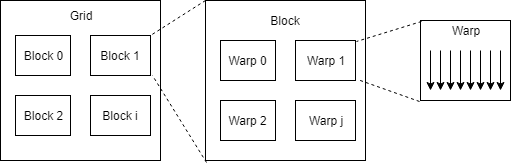
\includegraphics[width=0.9\linewidth]{Chapters/GPU/ThreadHierarchy.png}
  \captionof{figure}{Thread hierarchy}
  \label{fig:BSP}
\end{minipage}%
\begin{minipage}{.5\textwidth}
  \centering
  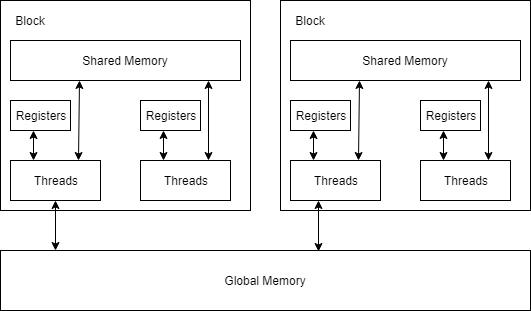
\includegraphics[width=0.9\linewidth]{Chapters/GPU/MemoryHierarchy.png}
  \captionof{figure}{Memory hierarchy}
  \label{fig:MapReduce}
\end{minipage}
\end{figure}

%\begin{figure}[!htb]
%    \centering
%    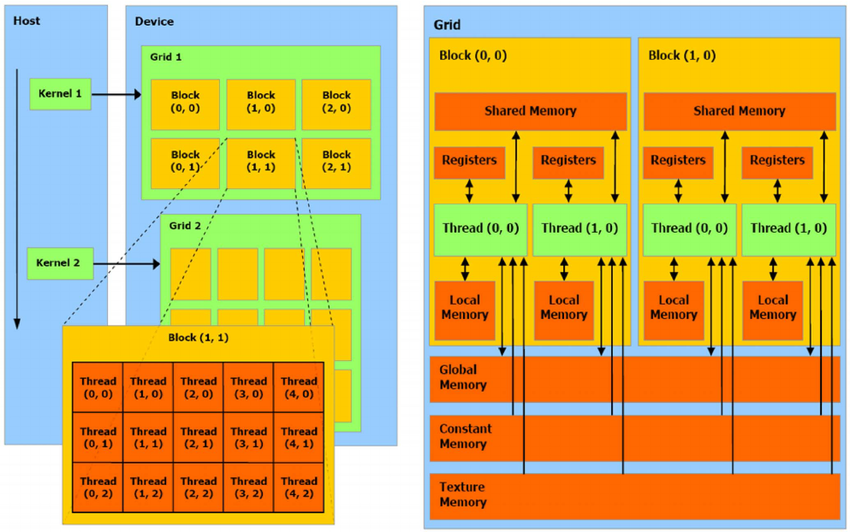
\includegraphics[width=\linewidth]{Chapters/GPU/CUDA-architecture.png} 
%    \caption{Schematization of GPU architecture - image extracted from Nobile et al.~\cite{nobile2014cutauleaping}, doi:10.1371/journal.pone.0091963.g001}
%\end{figure}

Beyond the thread hierarchy, GPU memory is organized into three ``main'' levels: global, shared/local and private with different sizes and speeds. The global memory is accessible from any thread in the grid, this is the equivalent of our external data source. It typically contains several GB of data and has a bandwidth of over 100GB/s. Shared memory is accessible only by threads being located within a same block, and thus linked to a streaming multiprocessor. It is much smaller, about 32KB, but is incredibly fast, it can peak up to 1300GB/s. Finally, private memory is only accessible within one warp. Its size and speed are not fixed since they can be located in different places, either in registers, shared or global memory, but for communication operations between members of the same warp, we can expect up to 7500GB/s.

Memory is also explicitly managed instead of what we found in an implicit cache\index{Cache} system (like a CPU). This aims to offer the possibility to take advantage of those for our particular problem through caching and prefetching policies which can be specifically designed according to algorithmic or application needs. At the same time, its handling is crucial to obtain the best performance possible~\cite{ueng2008cuda}. Most of the specific features proposed by those API are only dedicated to this aspect.

The programming work-flow of GPU computing is also different. It defines a host-device relationship between the CPU and GPU. This helps to take advantage of heterogenous computation. The principle is simple, a host program uploads the problem into the device (GPU memory), and then invokes a kernel passing the different parameters of the problem: the number of threads per block as well as the number of blocks, and the arguments of the program. The host program can either work in a synchronous or asynchronous manner, depending if the result from the GPU is currently needed for the next step or not. When the kernel has finished in the GPU, the result data is copied back from device to host~\cite{stone2010opencl}.

In practice, the essential difference with traditional programming is parallelism management. It is necessary to aim that the processings are the same for all threads. Only, it is not possible in all cases, either because the problem does not lend itself to it, or because the algorithm is not sufficiently adapted. Parallelism can then be controlled more precisely, first by dealing with the problem in blocks and if necessary by warps. By trying each time that there is a minimum of divergence between these different levels of parallelism.

The divergence in the computations is one of the biggest issues. Since an instruction is applied to the entire warp, this implies that each execution flow must be performed one after the other when there is a branching, with a mask indicating whether the results should be conserved or not. If everyone takes the same path, there are no such problems. The more branchings the code has, the slower it will be.

With this crucial aspect, care must be taken to consume the best available resources (registers or memories) in order to allow maximum parallelism and benefit from the locality of the data.

\subsection{Hardware considerations}

Many considerations come into account while implementing algorithms on GPU and which can have significant impact on the performances that will be achieved. We will try to remain as abstract as possible on problems that are highly technical. We must therefore be attentive, when programming, to various concepts. Achieving the maximum possible performance from these tools is often very difficult and it is best to keep different elements in mind. Algorithms can also be designed to rely on these underlying ideas.

\subsubsection{Coalesced\index{Coalesced} memory}

This notion refers to the ideal scenario of memory accesses where consecutive threads access to consecutive chunks of data. This access pattern helps the data prefetching and, thus, to increase the memory bandwidth, making the implementation more efficient. This also corresponds to the notion of blocks\index{Block} found in the external memory computation model. On the other side, irregular access patterns will lead to reduced performances~\cite{baskaran2008optimizing}.

Note that the term coalesced\index{Coalesced} is more specifically used when the memory address is aligned on a multiple of the entire cache\index{Cache} line and each thread accesses the element associated with its bank (small independant memory cell), the one linked to its identifier (more practically, this corresponds thus to the case mem[cache line size * k + thread identifier]). We will return to these notions in more details in a forthcoming chapter$^{[\ref{Accesses}]}$.

\subsubsection{Bank conflict}

% http://gpgpu.org/wp/wp-content/uploads/2013/09/08-opti-smem-instr.pdf

To speed up data access, shared memory is divided into small contiguous memory areas (about 4 bytes) called \textit{bank}. These units guarantee extremely fast accesses at the price of being able to process only one request at a time. So we also have to be cautious about \textit{bank conflicts} which occur when multiple threads attempt to access elements inside the same shared memory bank, those are then serialized leading to poor performances. The hardware splits a memory request with bank conflicts into as many separate conflict-free requests as necessary, decreasing throughput by a factor equal to the number of separate memory requests. The latest hardware versions are capable of broadcasting the data if they are located inside the same word, but accessing different words remains a problem~\cite{micikevicius2013performance}.

\subsubsection{Thread coarsening}

The granularity of the program can really affect the performances. Fine-grained tasks cause greater parallelism and therefore increases the speed-up, however more synchronization or scheduling strategies are also needed, which can have a negative impact on the performance. On the other hand, coarse-grained tasks have lower communication overhead, but often cause a load imbalance. It also allows to reuse same computation among the several tasks in unified manner or to reduce the overhead linked to the latency of the threads scheduling. Thread coarsening consists essentially to reduce the granularity of the algorithm to increase the amount of work per thread. Finding the good granularity is thus a really experimental tuning and the value of such process is usually limited due to the constantly reducing time required to launch a new kernel, schedule new warps or thanks to hardware improvements.

\subsubsection{Shared memory and caching}

The SIMT multiprocessors have fast private memory shared by all its cooperating threads. And threads are also layered in blocks which can all access to a share and common memory among all of them. Those two levels of cache\index{Cache} memory are orders of magnitude faster than the global device memory and thus can be exploided for peak performances.

\subsubsection{Padding}

Padding is the act to adjust the problem size on the level of the data to get a multiple of the block sizes. There is no more edge corner when considering the last elements of the problems. They fit tightly in the grid and thus require no more special treatment. Of course, the extra dummy data must not affect the original results. With padding, one can avoid putting conditional
statements in the kernel that would lead to unnecessary branching~\cite{navarro2014survey}.

\subsubsection{Branching}

Branching occurs when there are conditional statements in the kernel, both branches are then executed sequentially\index{Sequential}. It has a negative impact in performance and should be avoided whenever possible. The reason why branching occurs is because all threads within a warp execute in a lock-step mode and will run completely in parallel only if they follow the same execution path in the kernel code (SIMT\index{SIMT} computation); the result is thus discarded for the threads who did not take that path. If any conditional statement breaks the execution into two or more paths, then the paths are executed sequentially. Conditionals can be safely used if one can guarantee that the program will follow the same execution path for a whole warp. Additionally, we can use some logical operators which cause no branching and can be used to make disappear simple conditionals~\cite{harris2007parallel}.

\subsubsection{Memory use vs parallelism}

Finally, we said that the architecture conceptually allows an abstraction between the number of blocks and threads we launch and the real hardware capabilities. However, in practice, this is not totally the case, resources are scarce. The shared memory is very small (32KB) and can be shared by thousand threads; there are also only 256 registers but these condition the number of warps executable simultaneously on the same streaming multiprocessor, if we want to have in practice a thousand threads active, we should consume only 32 of them. Moreover, the more active threads there are, the more memory requests will be made and with them the number of cache\index{Cache} evictions. It is thus a real trade-off which must be carried out between the number of threads and blocks which one wants to execute and the resources which one can use.
